

\section{Method}
\label{sec:methods}

%We first describe our classifier for detecting split errors which is based on a convolutional neural network (CNN). We detail the CNN architecture, input features and the training method. We then describe how the same classifier can be used to detect merge errors and how we create potential corrections. The classifiers are integrated into an existing proofreading workflow as reported after. Finally, we explore an active label suggestion method which reorders the ranking obtained by our classifiers and maximizes the information gain provided by each potential correction.
\subsection{Split Error Detection}
\label{sec:spliterrordetection}

We build a split error classifier with output $p$ using a CNN to check whether an edge within an existing automatic segmentation is valid ($p=0$) or not ($p=1$). Rather than analyzing every input pixel, the classifier operates only on segment boundaries, which requires less pixel context and is faster. In contrast to Bogovic \etal~\cite{BogovicHJ13}, we work with 2D slices rather than 3D volumes. This enables proofreading prior or in parallel to a computationally expensive stitching and 3D alignment of individual EM images.

\paragraph{CNN Architecture.} Boundary split error detection is a binary classification task since the boundary is either correct or erroneous. However, in reality, the score $p$ is between 0 and 1. In connectomics, classification complexity arises from hundreds of different cell types, rather than from the classification decision itself. Intuitively, this yields a wider architecture with more filters rather than a deeper architecture with more layers. We explored different architectures---including residual networks~\cite{resnet}---with brute force parameter searches and precision and recall comparisons (see supplementary materials). Our final CNN configuration for split error detection has four convolutional layers, each followed by max pooling with dropout regularization to prevent overfitting due to limited training data (Fig.~\ref{fig:architecture}).

\paragraph{Classifier Inputs.} To train the CNN, we consider boundary context in the decision making process via a $75\times75$ patch over the center of an existing boundary. This size covers approximately $80\%$ of all boundaries in the 6~nm Mouse S1 AC3 Open Connectome Project dataset. If the boundary is not fully covered, we sample up to 10 non-overlapping patches along the boundary, and average the resulting scores weighted by the boundary length coverage per patch.
%\footnote{\scriptsize{\url{http://openconnectomeproject.org/}}}

Similar to Bogovic~\etal~\cite{BogovicHJ13}, we use grayscale image data, corresponding boundary probabilities, and a single binary mask combining the two neighboring labels as inputs to our CNN. However, we observed that the boundary probability information generated from EM images is often misleading due to noise or artifacts in the data. This can result in merge errors within the automatic segmentation. To better direct our classifier to train on the true boundary, we extract the border between two segments. Then, we dilate this border by 5 pixels to consider slight edge ambiguities as well as cover extra-cellular space, and use this binary mask as an additional input. This creates a stacked 4-channel input patch. Fig.~\ref{fig:cnn_inputs} shows examples of correct and erroneous input patches and their corresponding automatic segmentation and ground truth.

\begin{figure}[t]
\centering
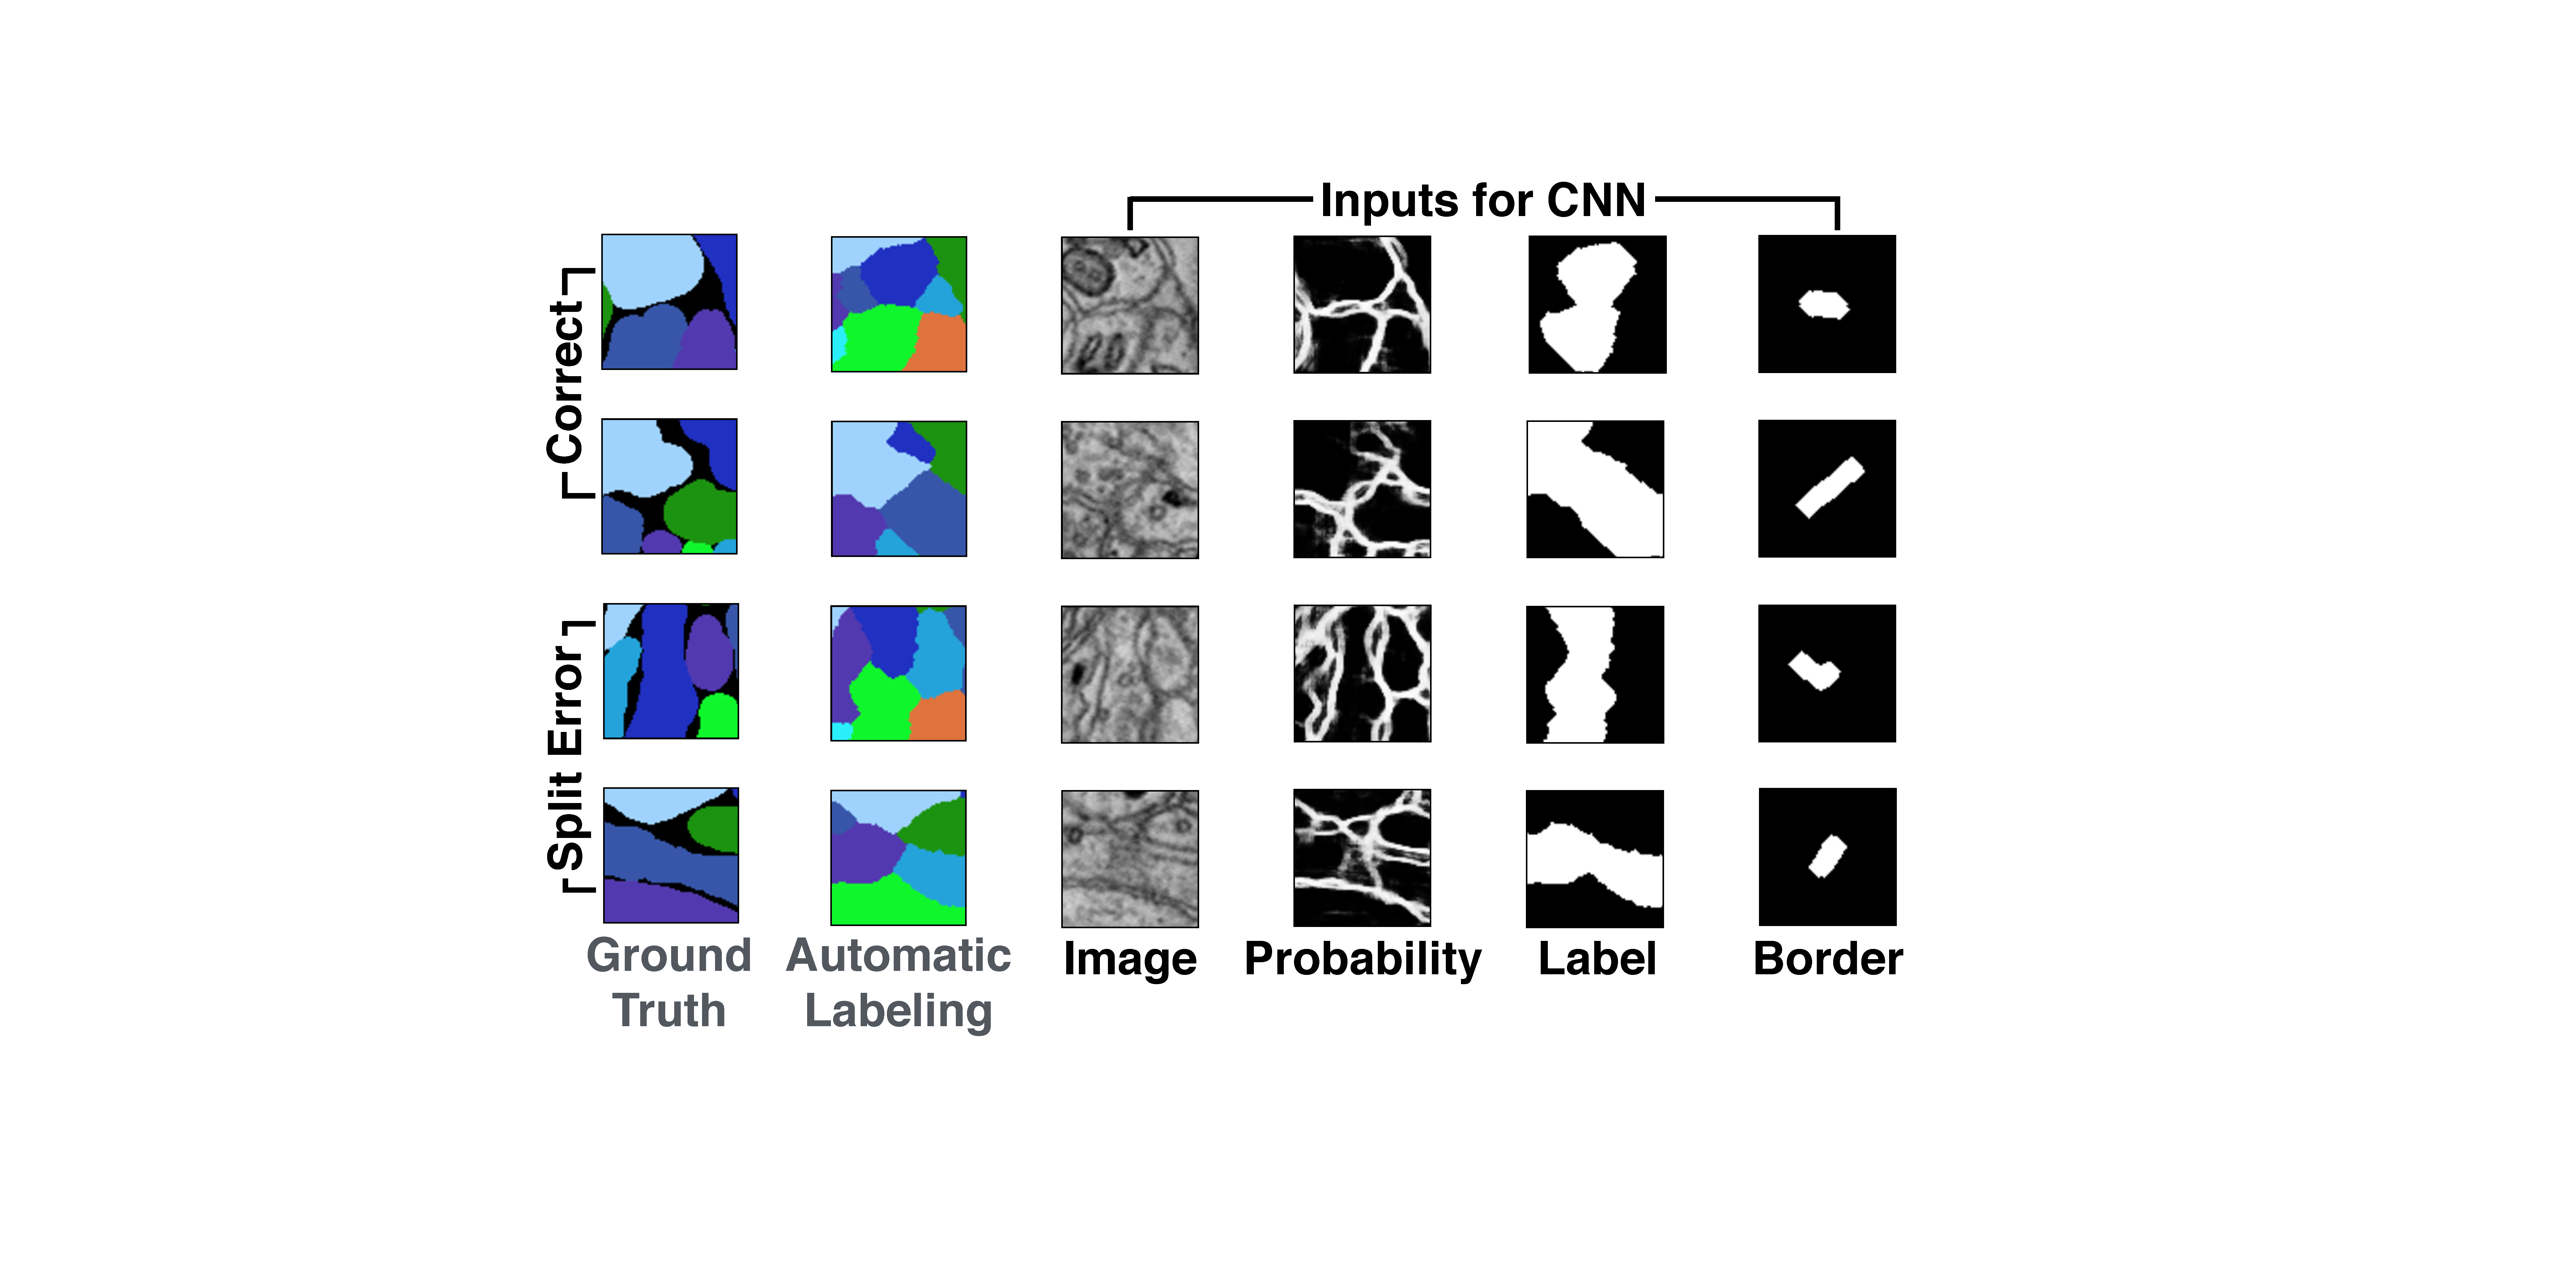
\includegraphics[width=\linewidth]{gfx/cnn_inputs.pdf}
\caption{Example inputs for learning correct splits and split errors (candidate segmentation versus the ground truth). Image, membrane probabilities, merged binary labels, and a dilated border mask provide 4-channel input patches.}
\label{fig:cnn_inputs}
\end{figure}


\subsection{Merge Error Detection}

Identification and correction of merge errors is more challenging than finding and fixing split errors, because we must look inside segmentation regions for missing or incomplete boundaries and then propose the correct boundary. However, we can reuse the same trained CNN for this task. 

\CHANGED{To find merge errors, we generate candidate splits within a label segment and use our split error classifier to rate them. If the classifier yields a result close to 0, meaning the candidate split is actually likely to be a correct one, then we assume that the label has been merged in error and that this candidate split will fix the merge error.}

%Similar to guided volume editing by Karimov~\etal~\cite{karimov_guided_volume_editing}, we generate potential borders within a segment. 

%For each segmentation label, we dilate the label by 20 pixel and generate 50 potential boundaries through the region by randomly placing watershed seed points at opposite sides of the label boundary. We perform watershed on the inverted grayscale EM image. This yields 50 candidate splits.
\CHANGED{For each segmentation label, we generate 50 potential boundaries through the region by randomly placing watershed seed points at opposite sides of the label boundary. As preprocessing, we dilate the label by 20 pixel which is motivated by our observation that the generated splits tend to attach to real membrane boundaries. These boundaries are then individually rated using our split error classifier.}

%We perform watershed on the inverted grayscale EM image. This yields 50 candidate splits. Prior to watershed, we dilate the label by 20 pixel which is motivated by our observation that the generated splits tend to attach to real membrane boundaries. These boundaries are then individually rated using our split error classifier. 

\CHANGED{Fig. \ref{fig:merge_error} illustrates this procedure. Pseudo code is available as supplemental material to promote understanding.}

%For this, we invert the probability score such that a correct split (previously encoded as $p=0$) is most likely a candidate for a merge error (now encoded as $p=1$). In other words, if a generated boundary is ranked as correct, it probably should be in the segmentation. Fig. \ref{fig:merge_error} illustrates this procedure. Pseudo code is available as supplemental material to promote understanding.

\begin{figure}[t]
\centering
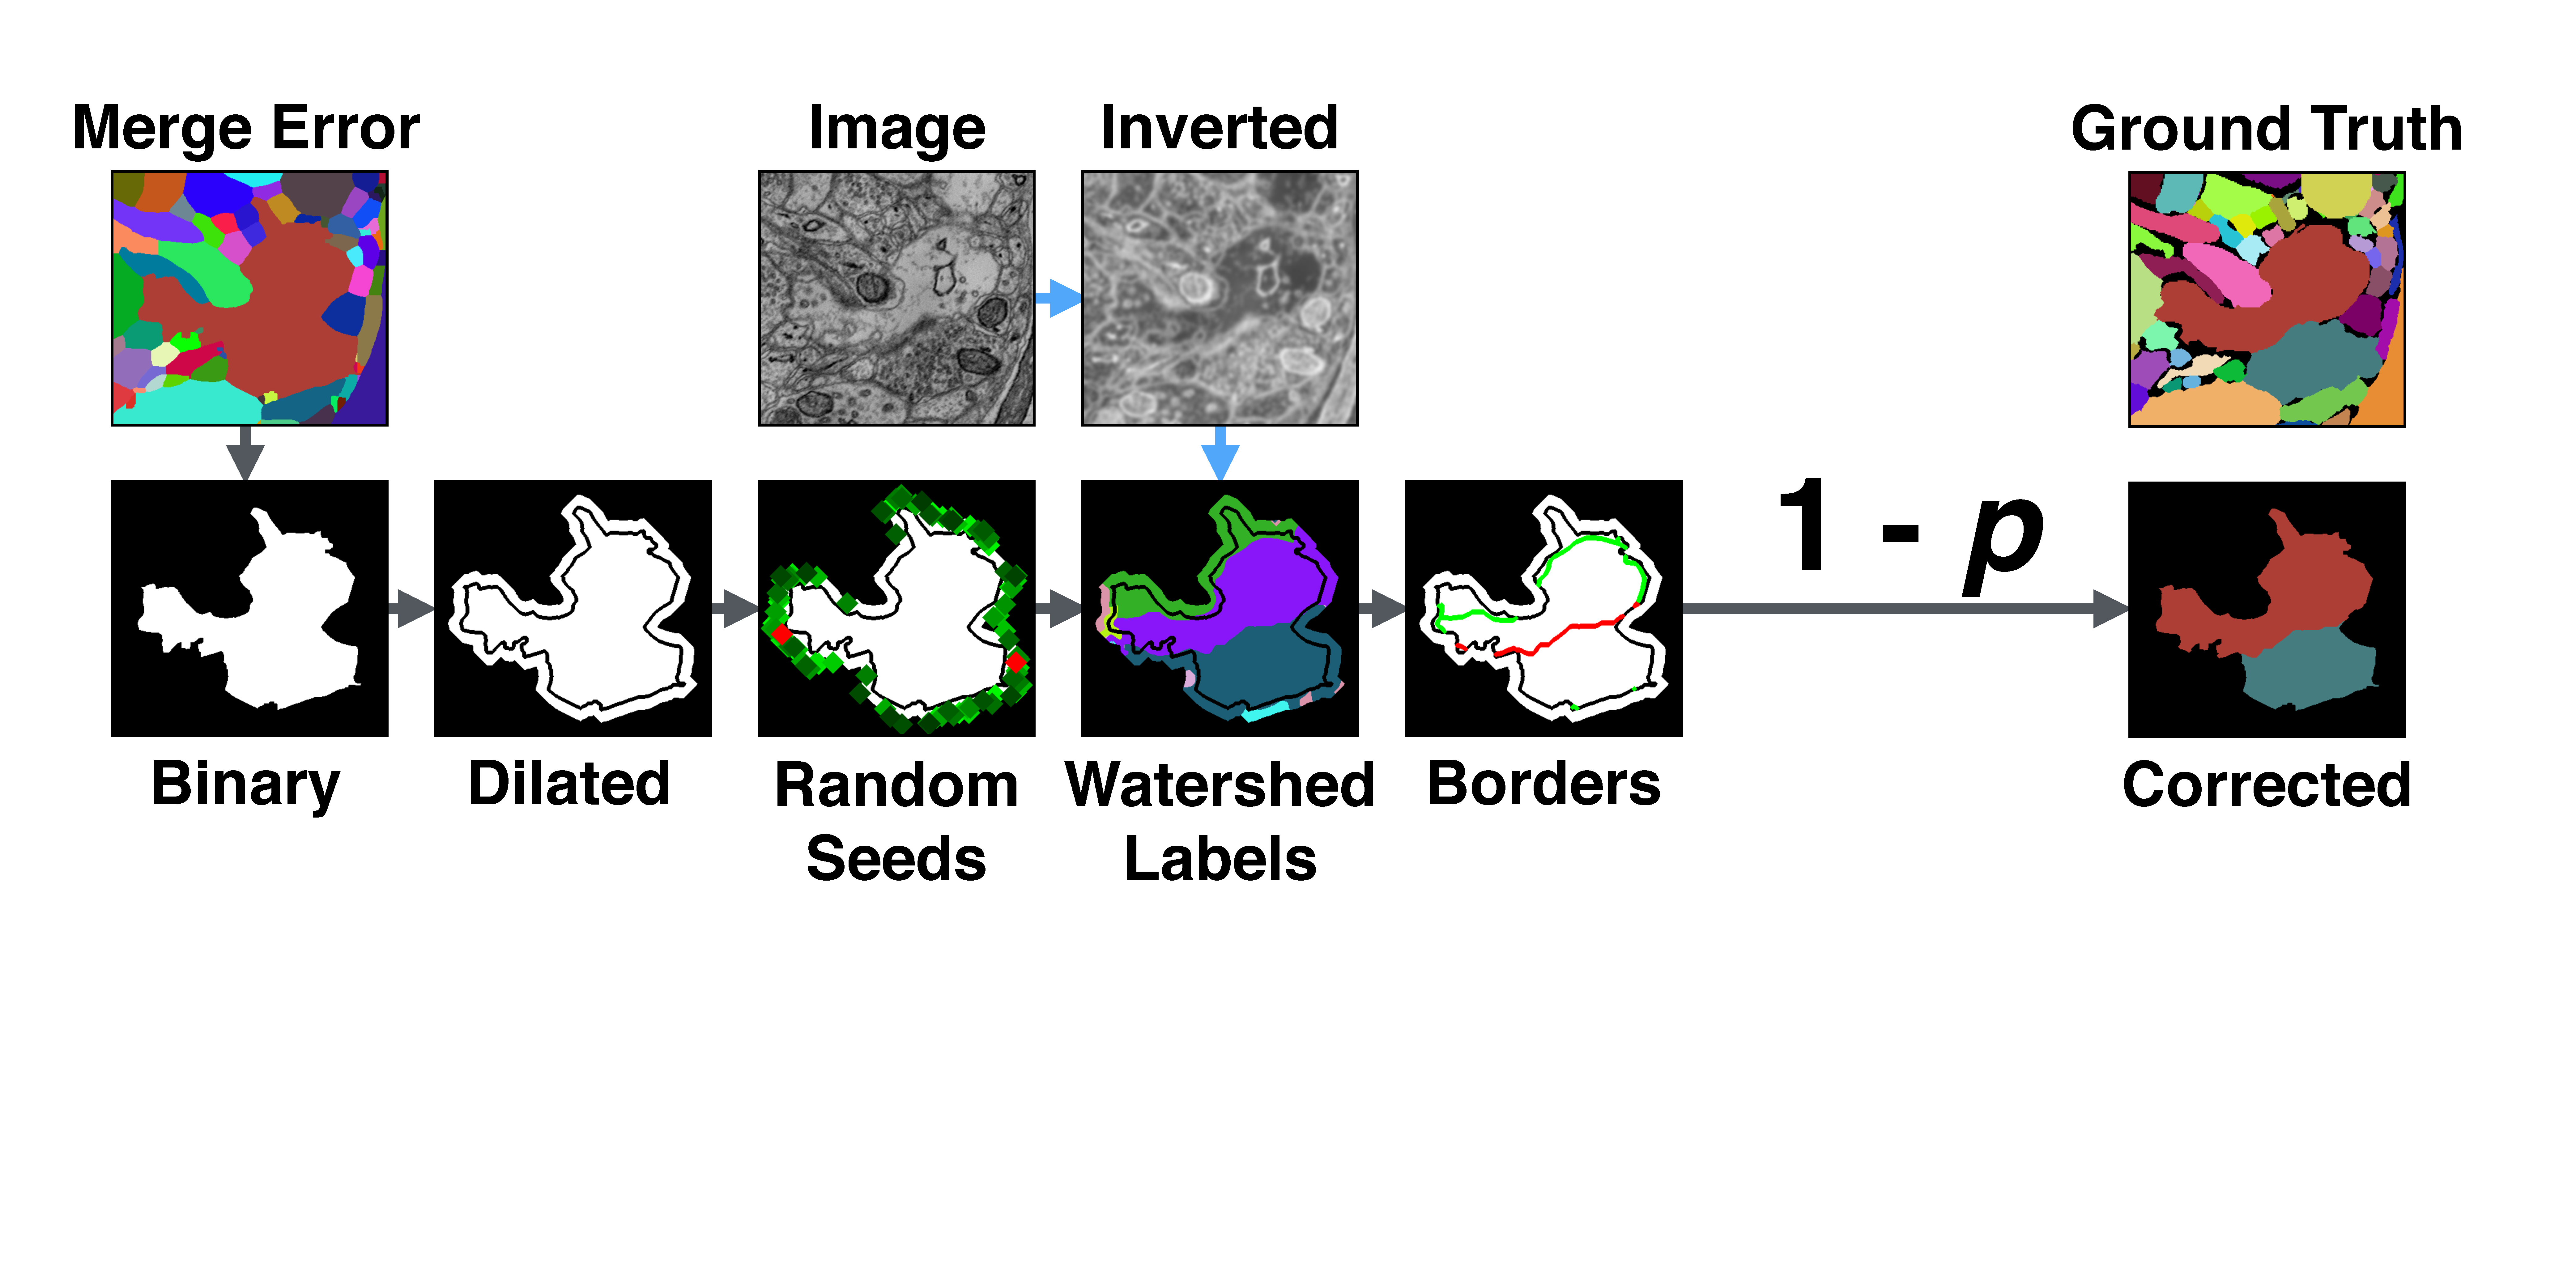
\includegraphics[width=\linewidth]{gfx/merge_error_v6.pdf}
\caption{Merge error detection: Potential borders are generated using inverted images by randomly placing watershed seeds (green) on the boundary of a dilated segment. The best ranked seeds and border (both in red) result in the shown error correction.}
%Merge errors are identified by generating randomly-seeded watershed borders within a dilated label segment. Then, each border is individually rated using the split error CNN by inverting the probability score. A confident rating for a correct split most likely indicates the missing border of the merge error, and can be used to correct the labeling.}
\label{fig:merge_error}
\end{figure}

\subsection{Error Correction}
\label{sec:errorcorrection}

We combine the proposed classifiers to perform corrections of split and merge errors in automatic segmentations. For this, we first perform merge error detection for all existing segments in a dataset and store the inverted rankings $1-p$ as well as potential corrections. After that, we perform split error detection and store the ranking $p$ for all neighboring segments in the segmentation. Then, we sort the merge and split error rankings separately from highest to lowest. For error correction, first we loop through the potential merge error regions and then through the potential split error regions. During this process, each error is now subject to a yes/no decision which can be provided in different ways:

\paragraph{Selection oracle.} If ground truth data is available, the selection oracle \textit{knows} whether a possible correction improves an automatic segmentation. This is realized by simply comparing the outcome of a correction using a defined measure. The oracle only accepts corrections which improve the automatic segmentation---others get
discarded. This is guided proofreading with a perfect user, and allows us to assess the upper limit of improvements.

\paragraph{Automatic selection with threshold.} The decision whether to accept or reject a potential correction is taken by comparing rankings to a threshold $p_t$. If the inverted score $1-p$ of a merge error is higher than a threshold $1-p_t$, the correction is accepted. Similarly, a correction is accepted for a split error if the ranking $p$ is higher than $p_t$. Our experiments have shown that the threshold $p_t$ is the same for merge and split errors for a balanced classifier that has been trained on equal numbers of correct and error patches.

\paragraph{Forced choice setting.} We present a user with the choice to accept or reject a correction. All potential split errors are seen. Inspecting all merge errors is not possible for users due to the sheer amount of generated borders. Therefore, we only present merge errors that have a probability threshold higher than $1-p_t$.

\noindent \newline In all cases, a decision has to be made to advance to the next possible erroneous region. If a merge error correction was accepted, the newly found boundary is added to the segmentation data. This partially updates the merge error and split error ranking with respect to the new segment. If a split error correction was accepted, two segments are merged in the segmentation data and the disappearing segment is removed from all error rankings. Then, we perform merge error detection on the now larger segment and update the ranking. We also update the split error rankings to include all new neighbors, and re-sort. The error with the next highest ranking then forces a choice.

\subsection{User Interface}

We integrate guided proofreading into an existing large data connectomics workflow. The web-based system is designed with a novice-friendly user interface (Fig.~\ref{fig:ui}). We show the current labeling of a cell boundary outline and its proposed correction overlayed on EM image data. The user cannot distinguish the current labeling from the proposed correction to avoid selection bias. We also show a solid overlay of the current and the proposed labeling. In addition, we show the image without overlays to provide an unoccluded view. User interaction is simple and involves one mouse click on either the current labeling or the correction. After interaction, the next potential error is shown.

\begin{figure}[t]
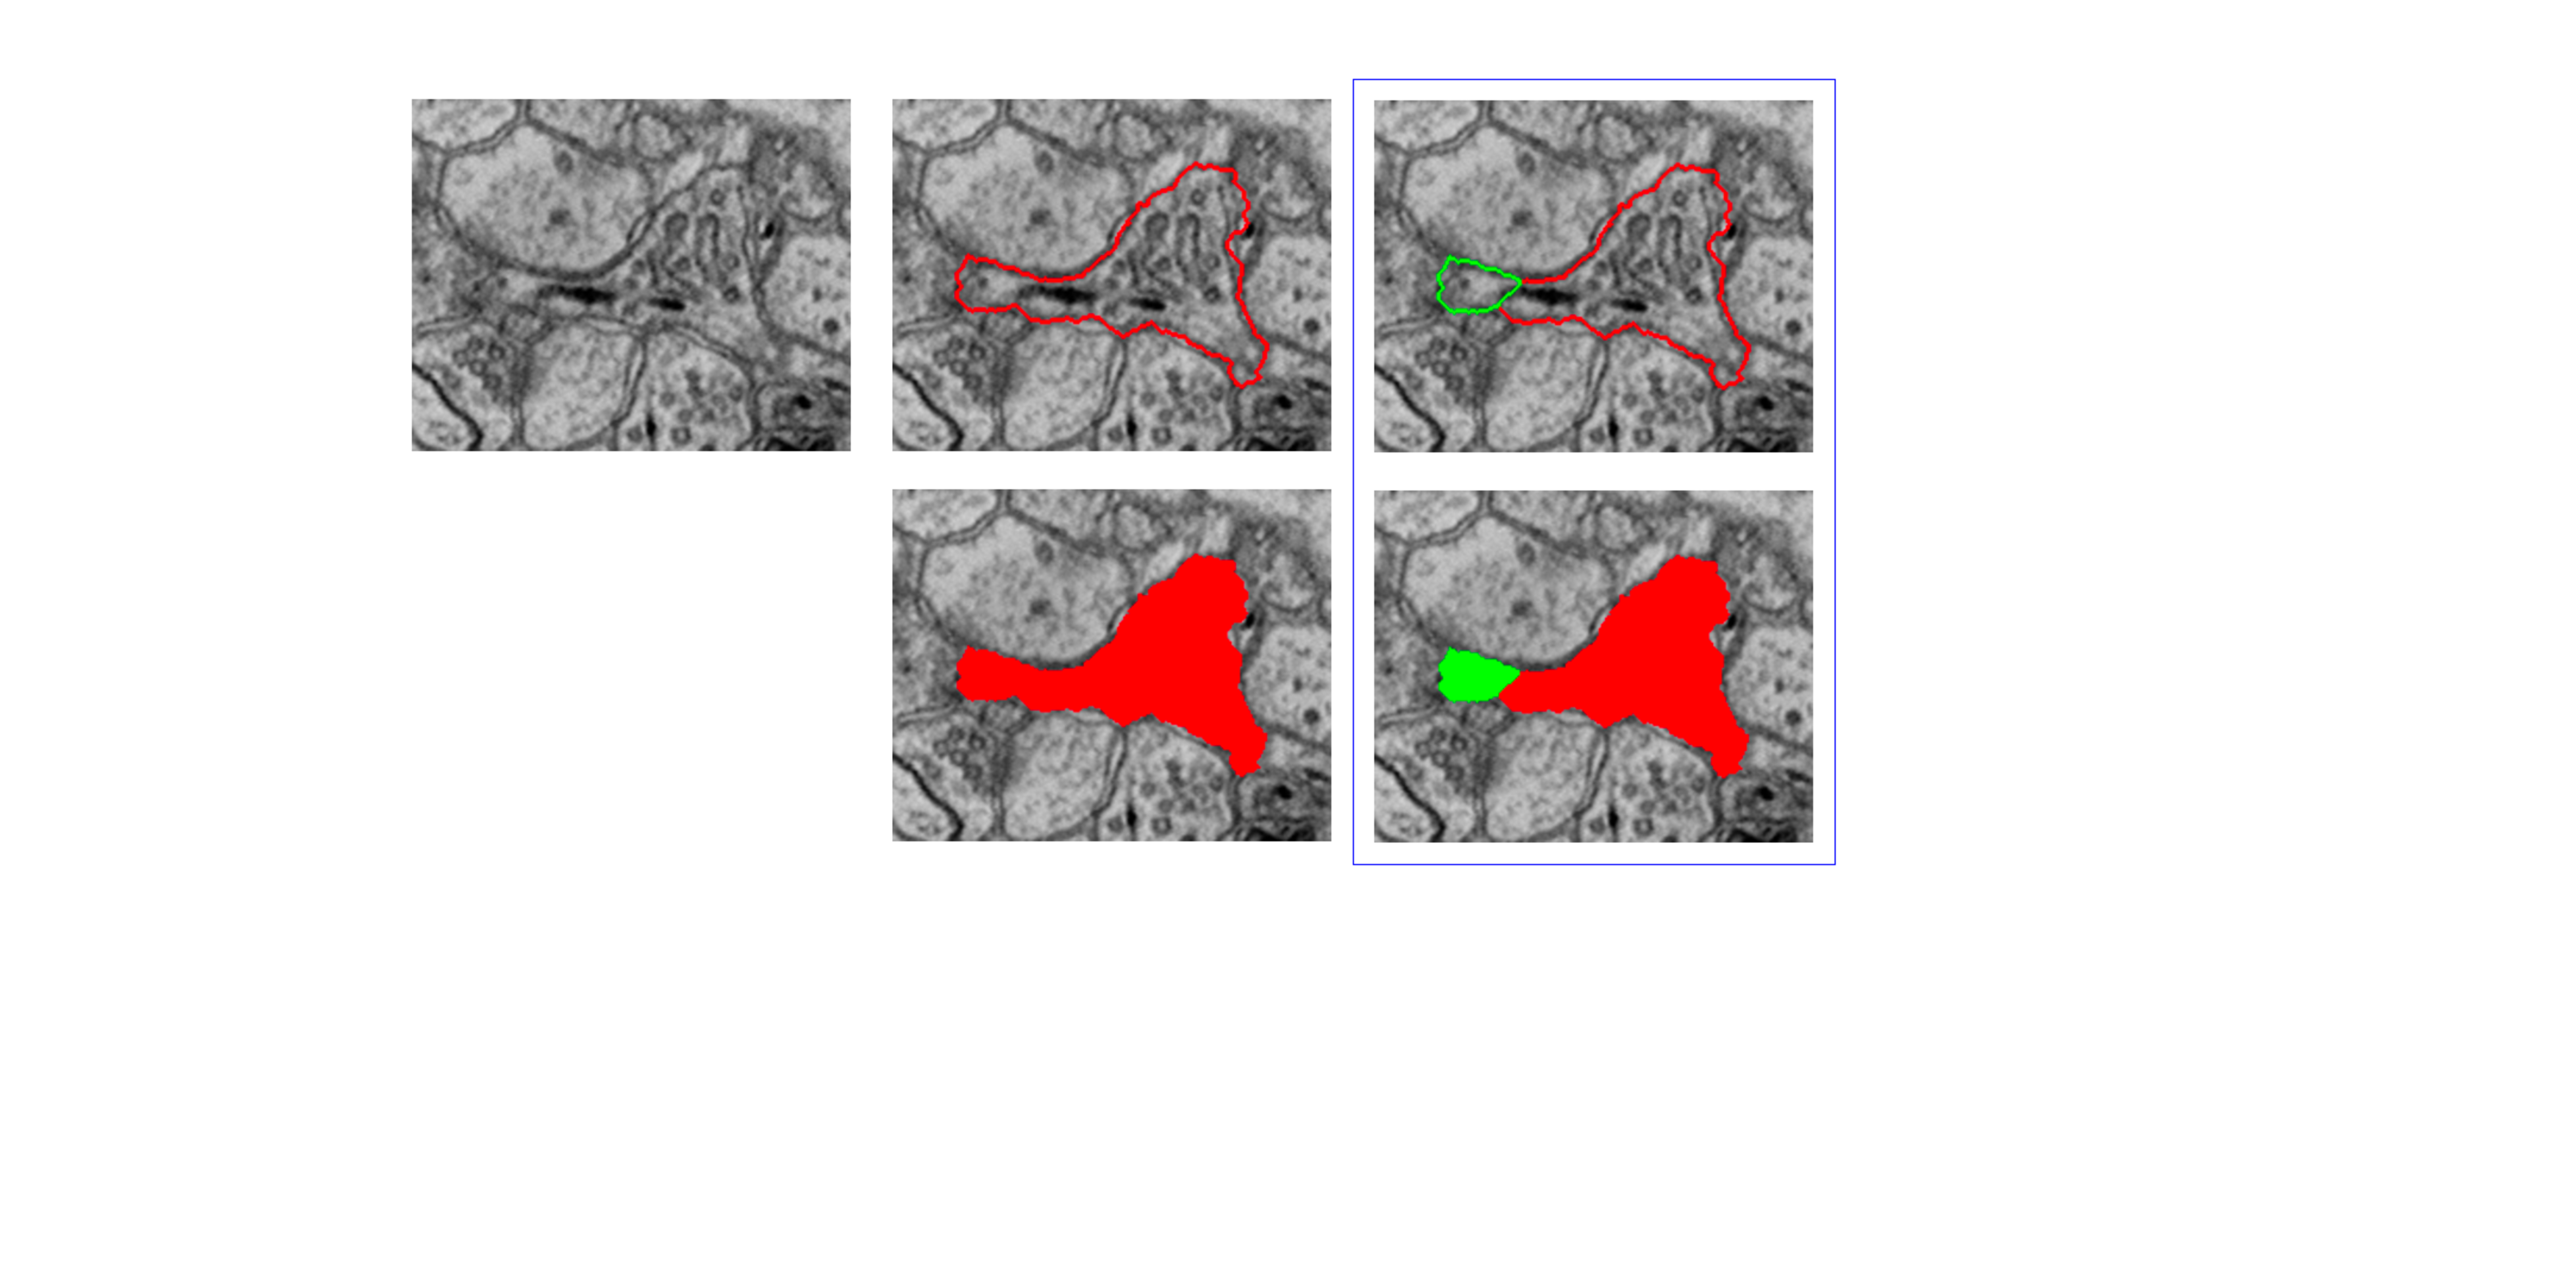
\includegraphics[width=\linewidth]{gfx/user_interface_split.pdf}
\caption{User interface. A candidate error region is shown on the left. The user must choose between the region being a split error which needs correcting (center) or not (right). Confirming the choice advances to the next potential error.} % Hovering highlights the current selection with a blue border, and a}
\label{fig:ui}
\end{figure}

%
%\subsection{Active Label Suggestion}
%
%In an interactive setting, one way to present patches to the user for proofreading is to order them by the confidence probability of the GP classifier. However, in an active learning setting, where the network is retrained repeatedly on new label evidence, this approach is less likely to decrease segmentation error as, with the new labels, we are only reinforcing what the network already has a high confidence in.
%Instead, we apply active label suggestion to guide the user into labeling patches which will be more informative to retraining, and so overall decrease VI faster within the proofreading cycle of label $\rightarrow$ train $\rightarrow$ label. For each patch, we remove the softmax classification layer and look at the activation weights associated with the last dense layer. These become a high-dimensional feature vector. Then, we adapt Anon~\etal~\cite{ANON} to provide label suggestions based on features from the learned CNN, which is based on maximizing the average information gain provided by a candidate patch to label.
%A second consideration is that each patch labeled by the user provides evidence to other patches, e.g., correcting a split error redefines an entire boundary, from which multiple candidate patch labelings could have been drawn. As such, when the user labels a patch, we consider all `knock-on' effect patches as also being labeled, and feed these into the active label suggestion system similarly.
%In section \ref{sec:evaluation}, we report the difference in performance from using active label suggestion rather than confidence ordering when presenting patches to the user. These results are without retraining the network after new labelings: this should improve results, but would have to be batched to reduce computational load; hence, we leave this for future work.
